\section{Results \& Discussion}

A plot of the magnetic field from the earth is shown in figure \ref{fig:earth}.

\begin{figure}[htb]
	\centering
	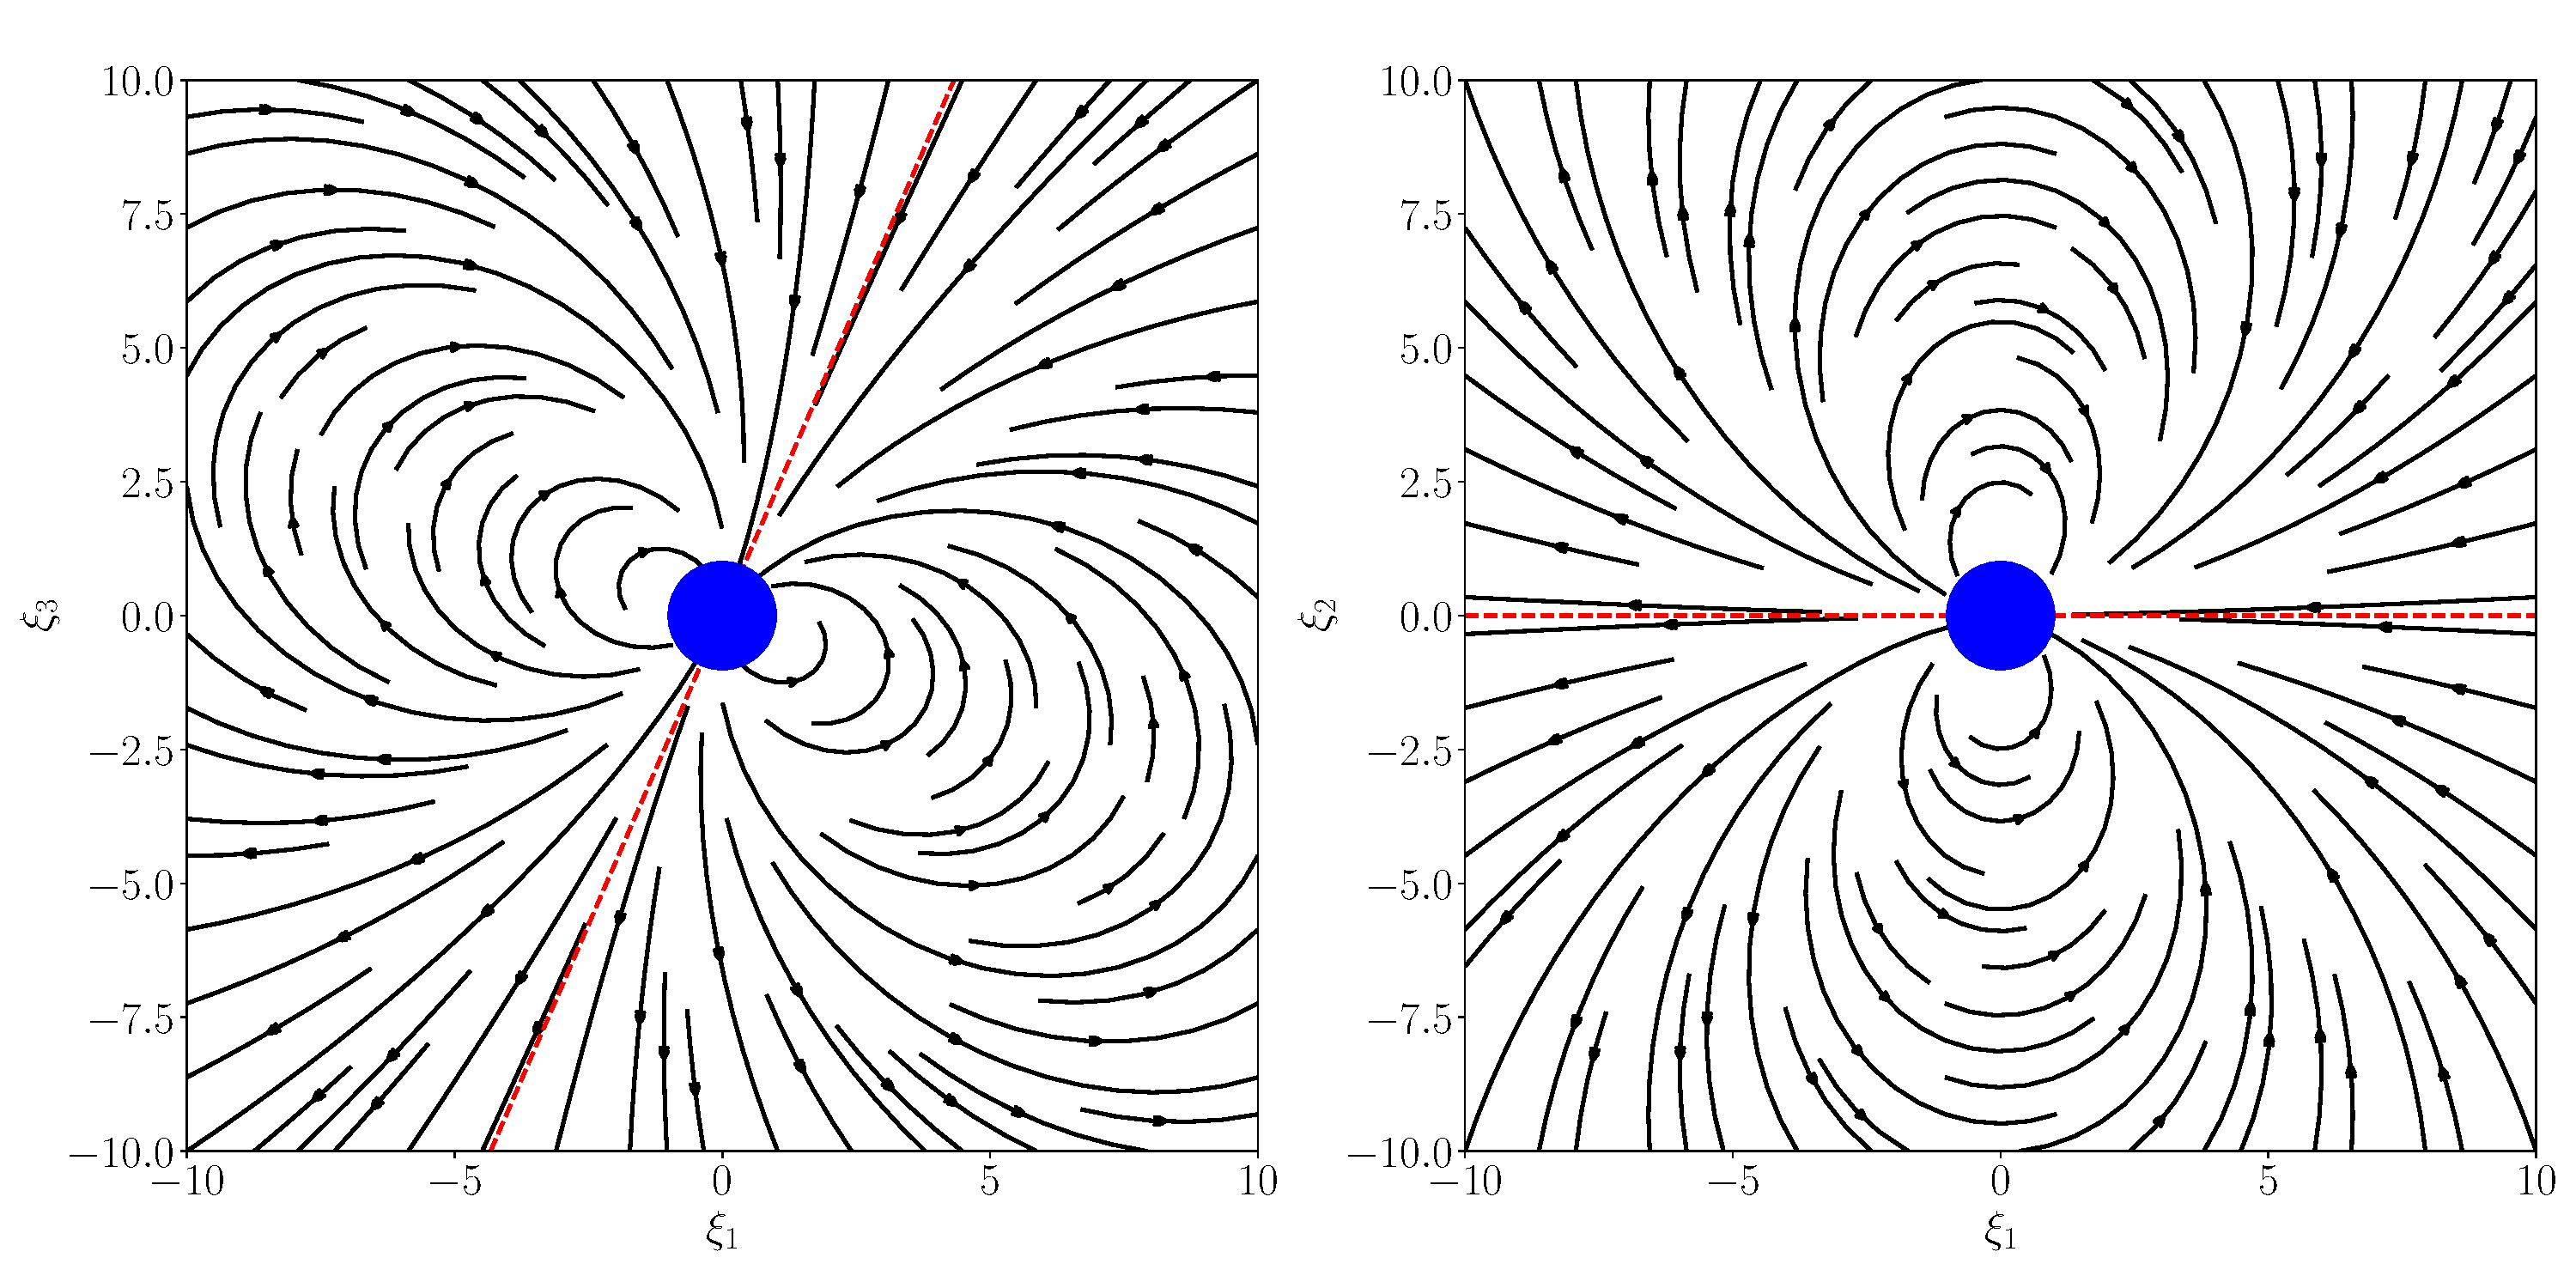
\includegraphics[width=\columnwidth]{../fig/earth.pdf}
	\caption{Magnetic field from earth. The tilt of the ecliptic with respect to the equator is $23.5^\circ$ \cite{https://doi.org/10.1029/2012JA018056}.}
	\label{fig:earth}
\end{figure}

When sending particles far from the earth towards it they start spiralling around the field lines. This is consistent with the fact that the magnetic force acts perpendicular to the trajectory, and the fact that the motion along $\mathbf{B}$ is uniform in the first approximation, as considered in section \ref{sec:motion}. This is shown in figure \ref{fig:fast_part} and \ref{fig:slow_part}. 
%Also apparent from these plots is that the gyration radius is larger when the particles are sent towards earth with larger speed. 
Moreover, in figure \ref{fig:fast_part} we observe a clockwise drift around the equator, as predicted by equation \eqref{eq:v_grad} and \eqref{eq:v_curv}.

\begin{figure}[h!]
	\centering
	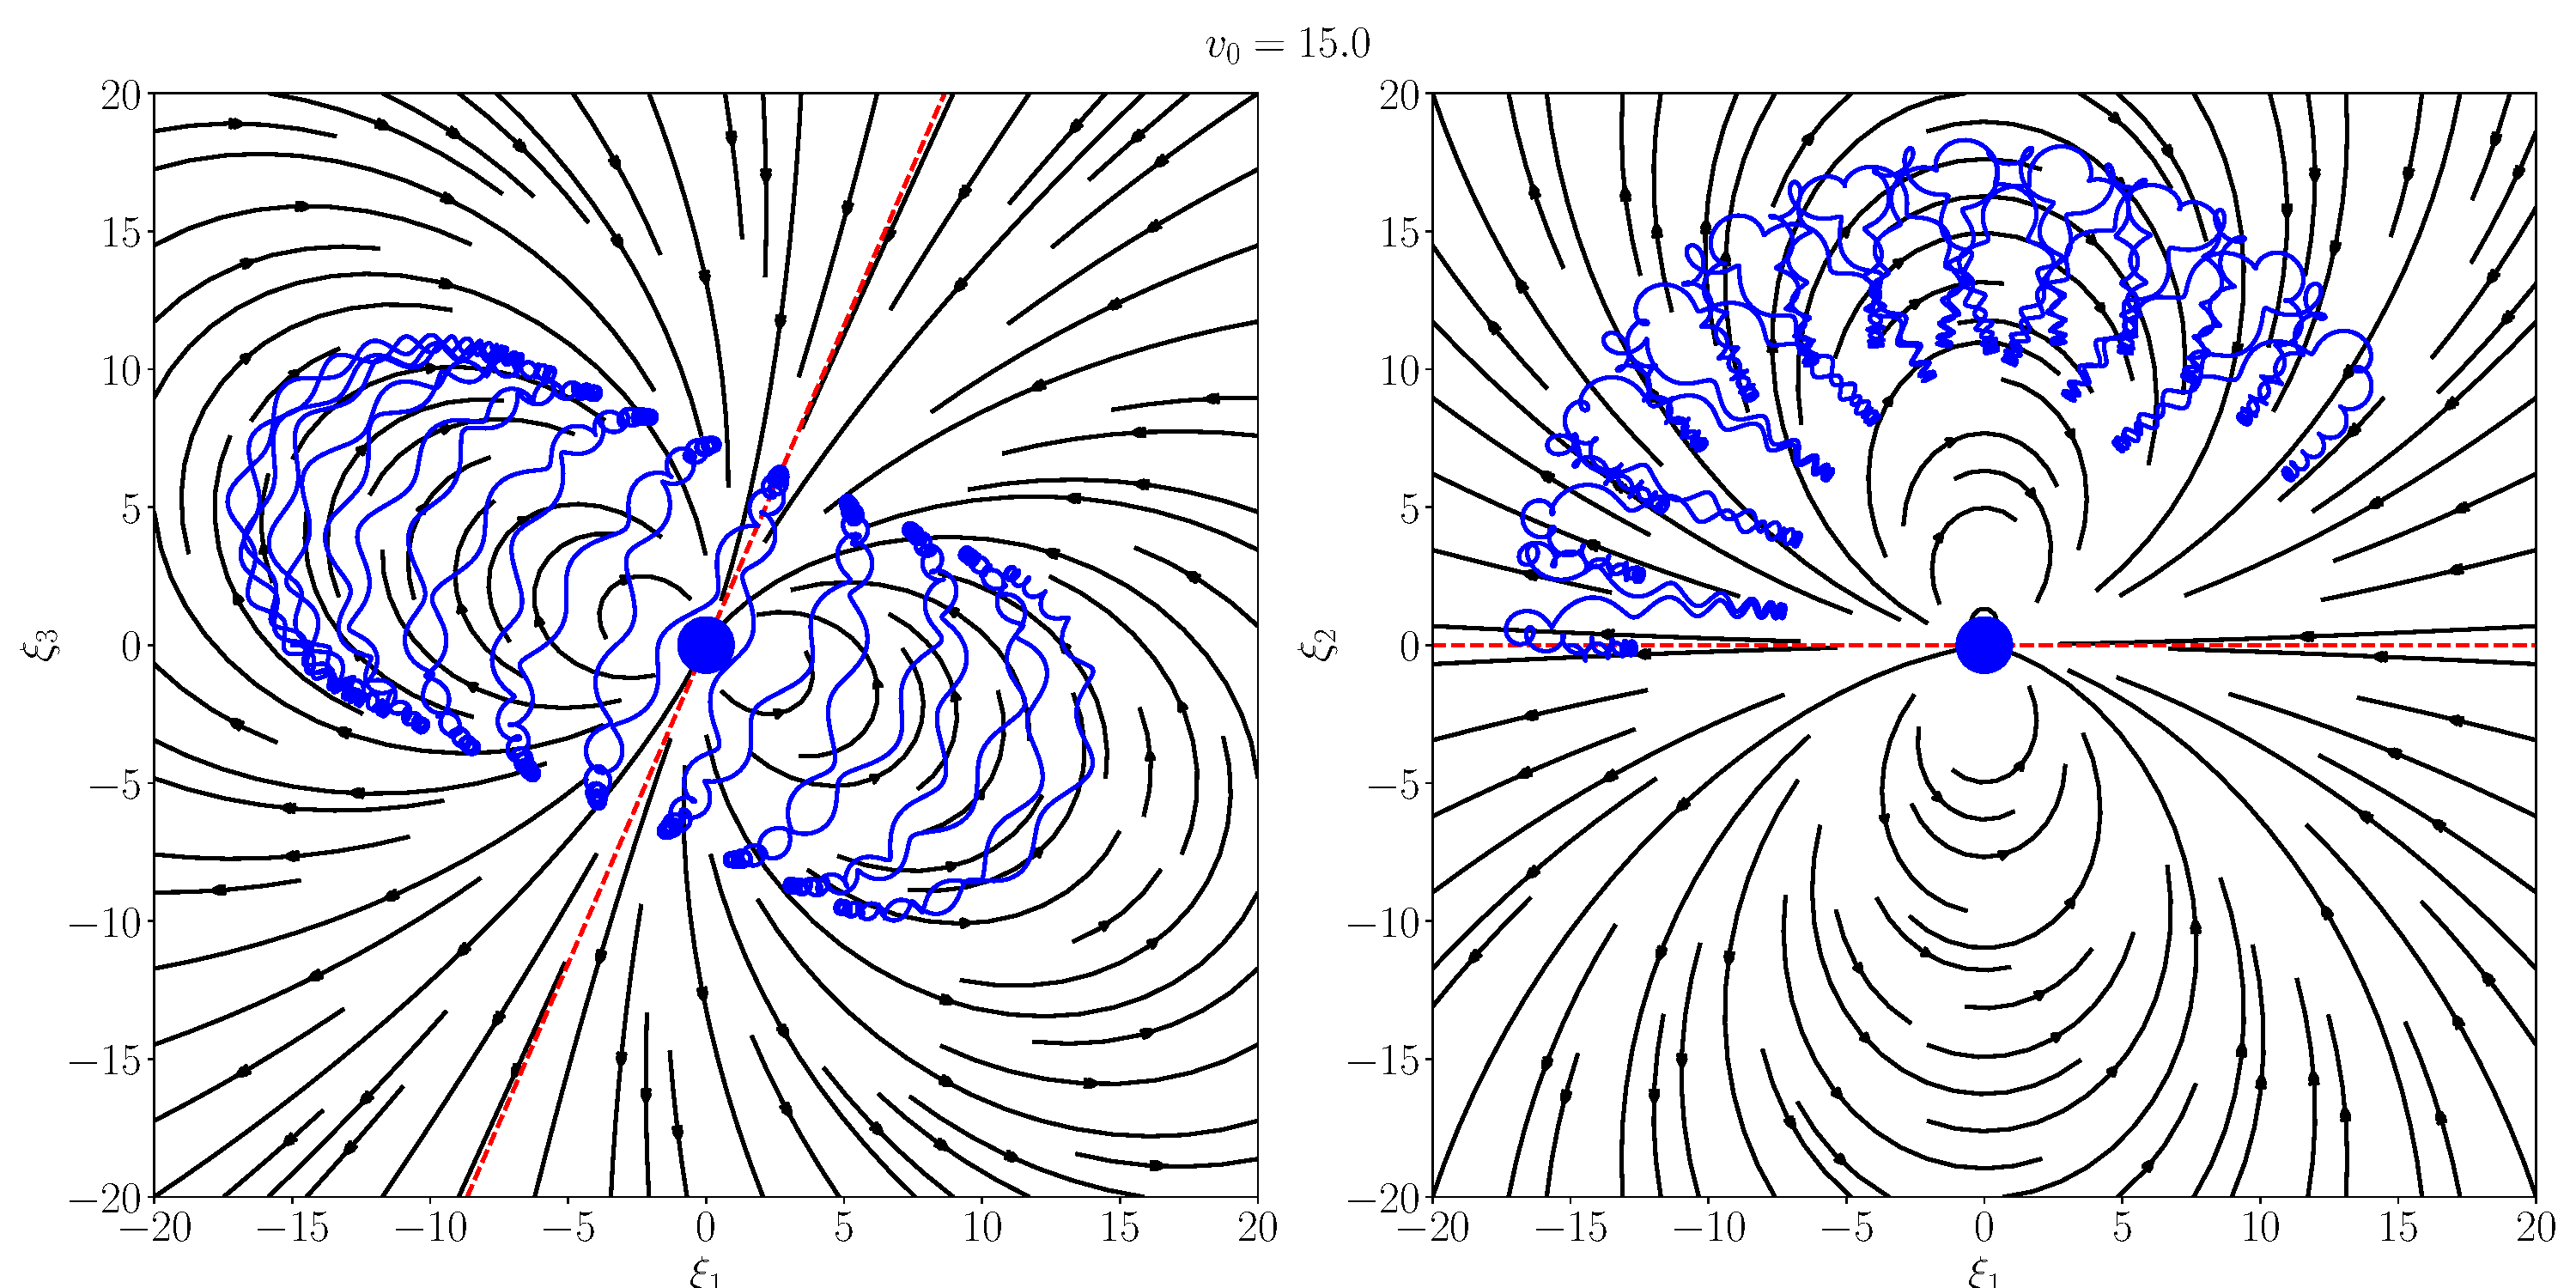
\includegraphics[width=\columnwidth]{../fig/earth_traj_fast.pdf}
	\caption{Particle sent towards the earth with high solar wind velocity.}
	\label{fig:fast_part}
\end{figure}

The trajectories of particles sent towards earth at different heights $z$ ($\xi_3$) is shown in figure \ref{fig:different_z}.

\begin{figure}[htb]
	\centering
	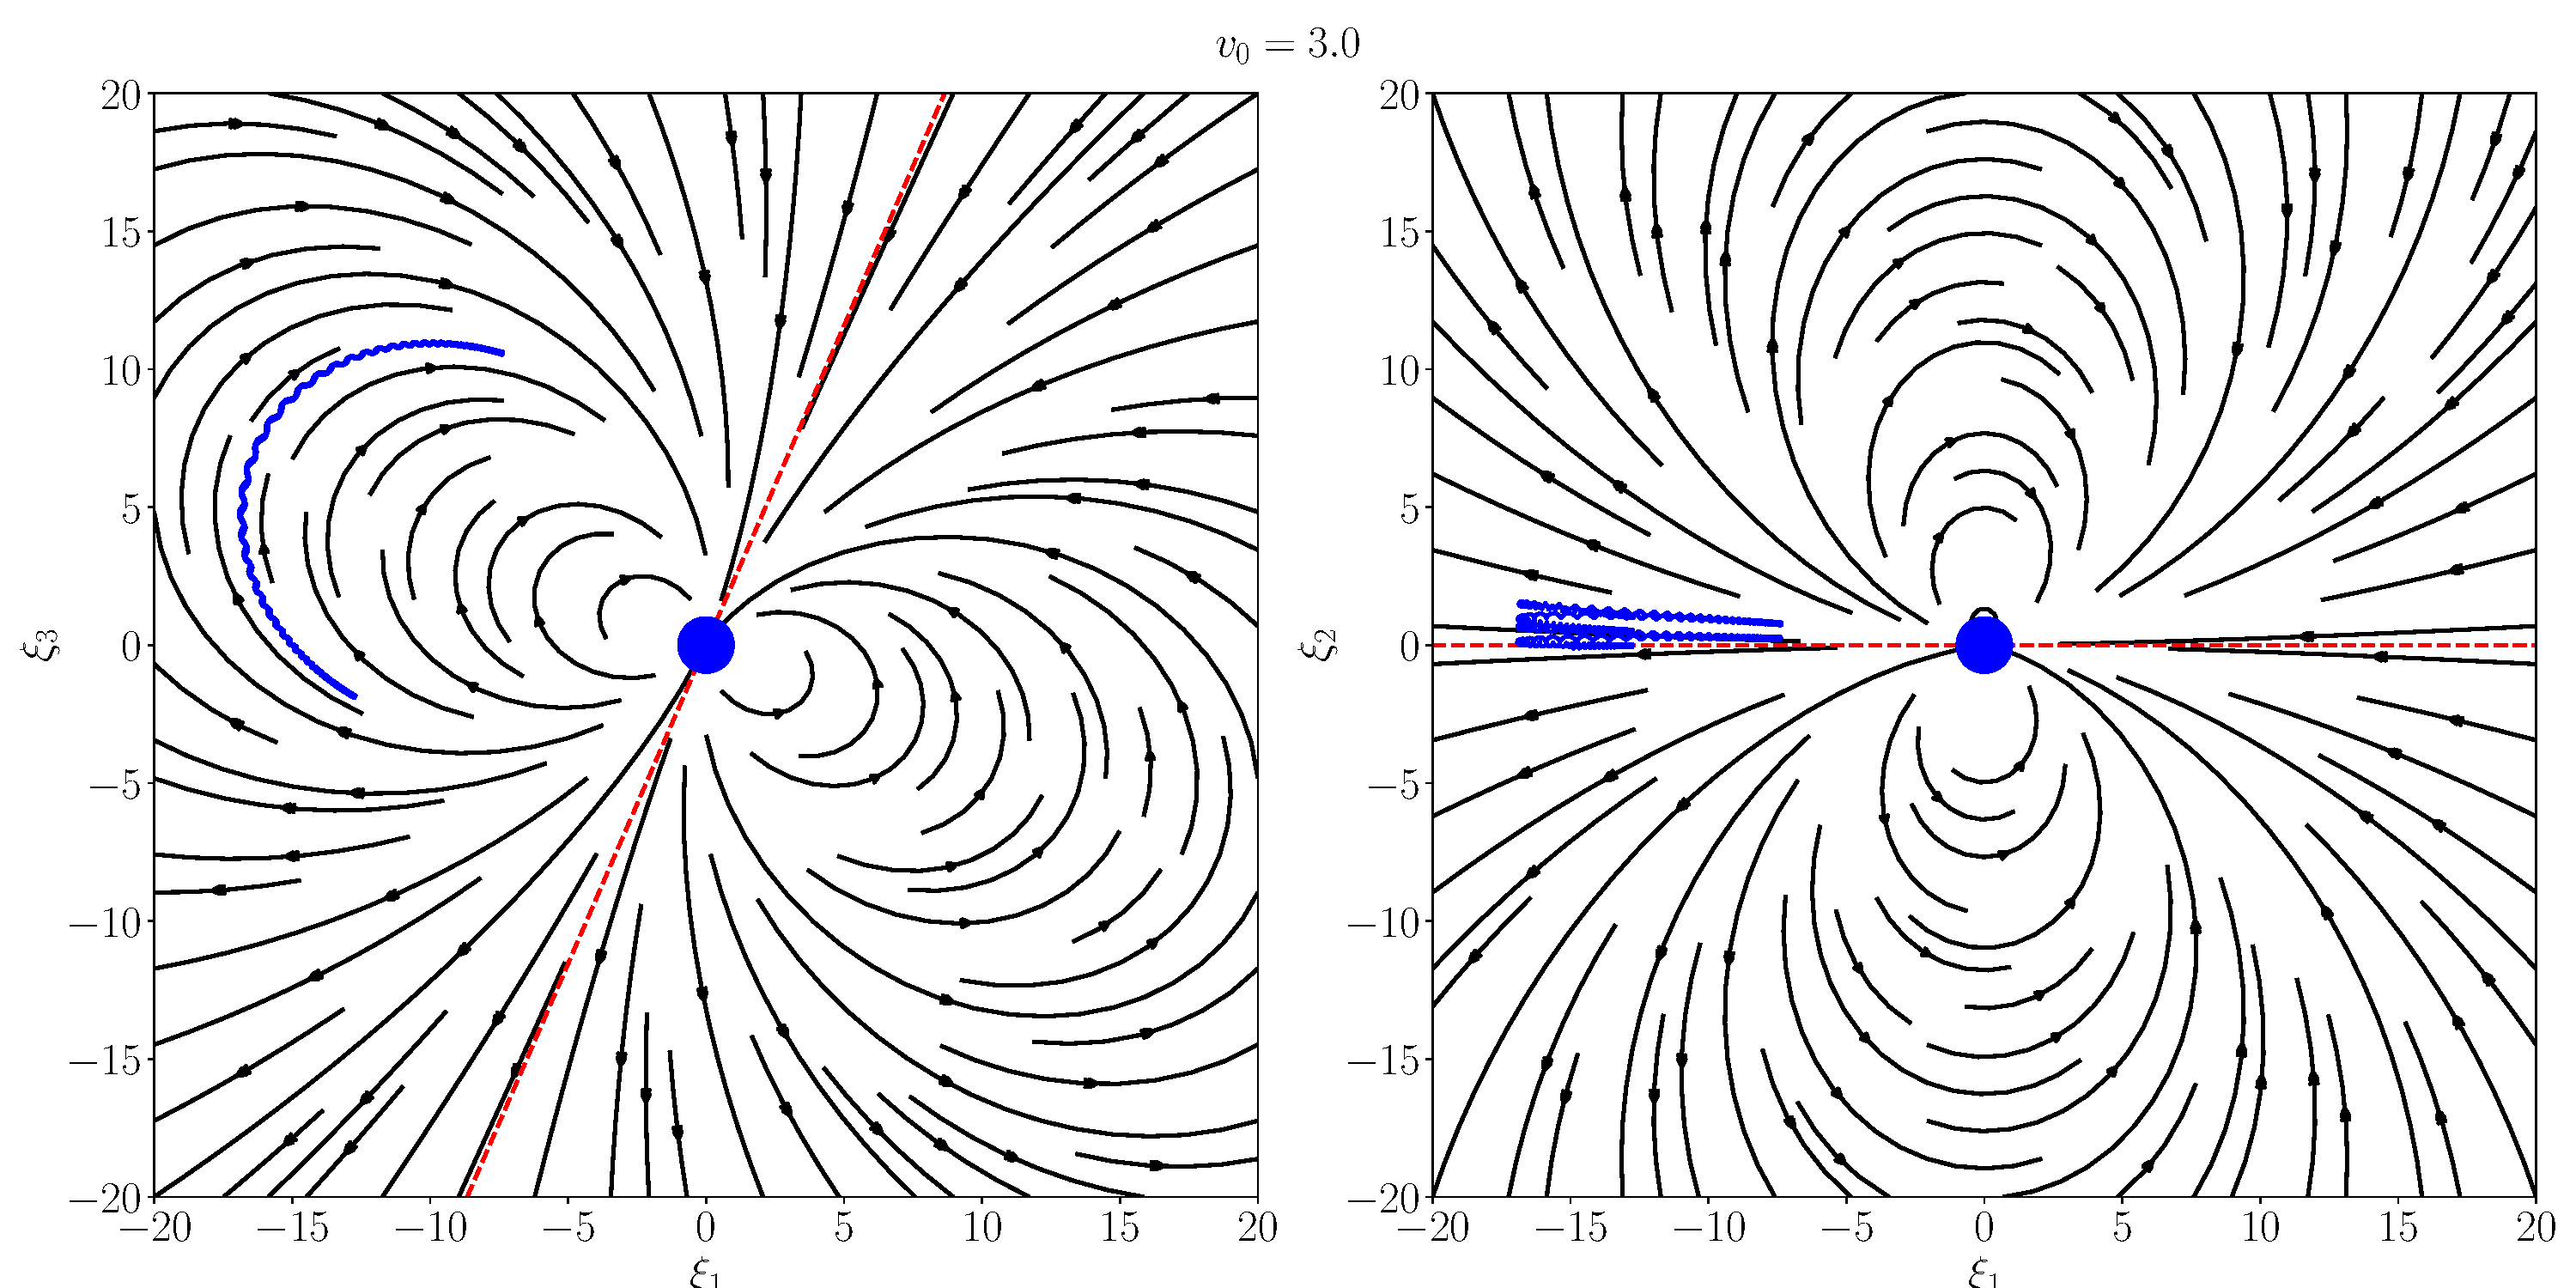
\includegraphics[width=\columnwidth]{../fig/earth_traj_slow.pdf}
	\caption{Particle sent towards the earth with typical solar wind velocity.}
	\label{fig:slow_part}
\end{figure}
\begin{figure}[h!]
	\centering
	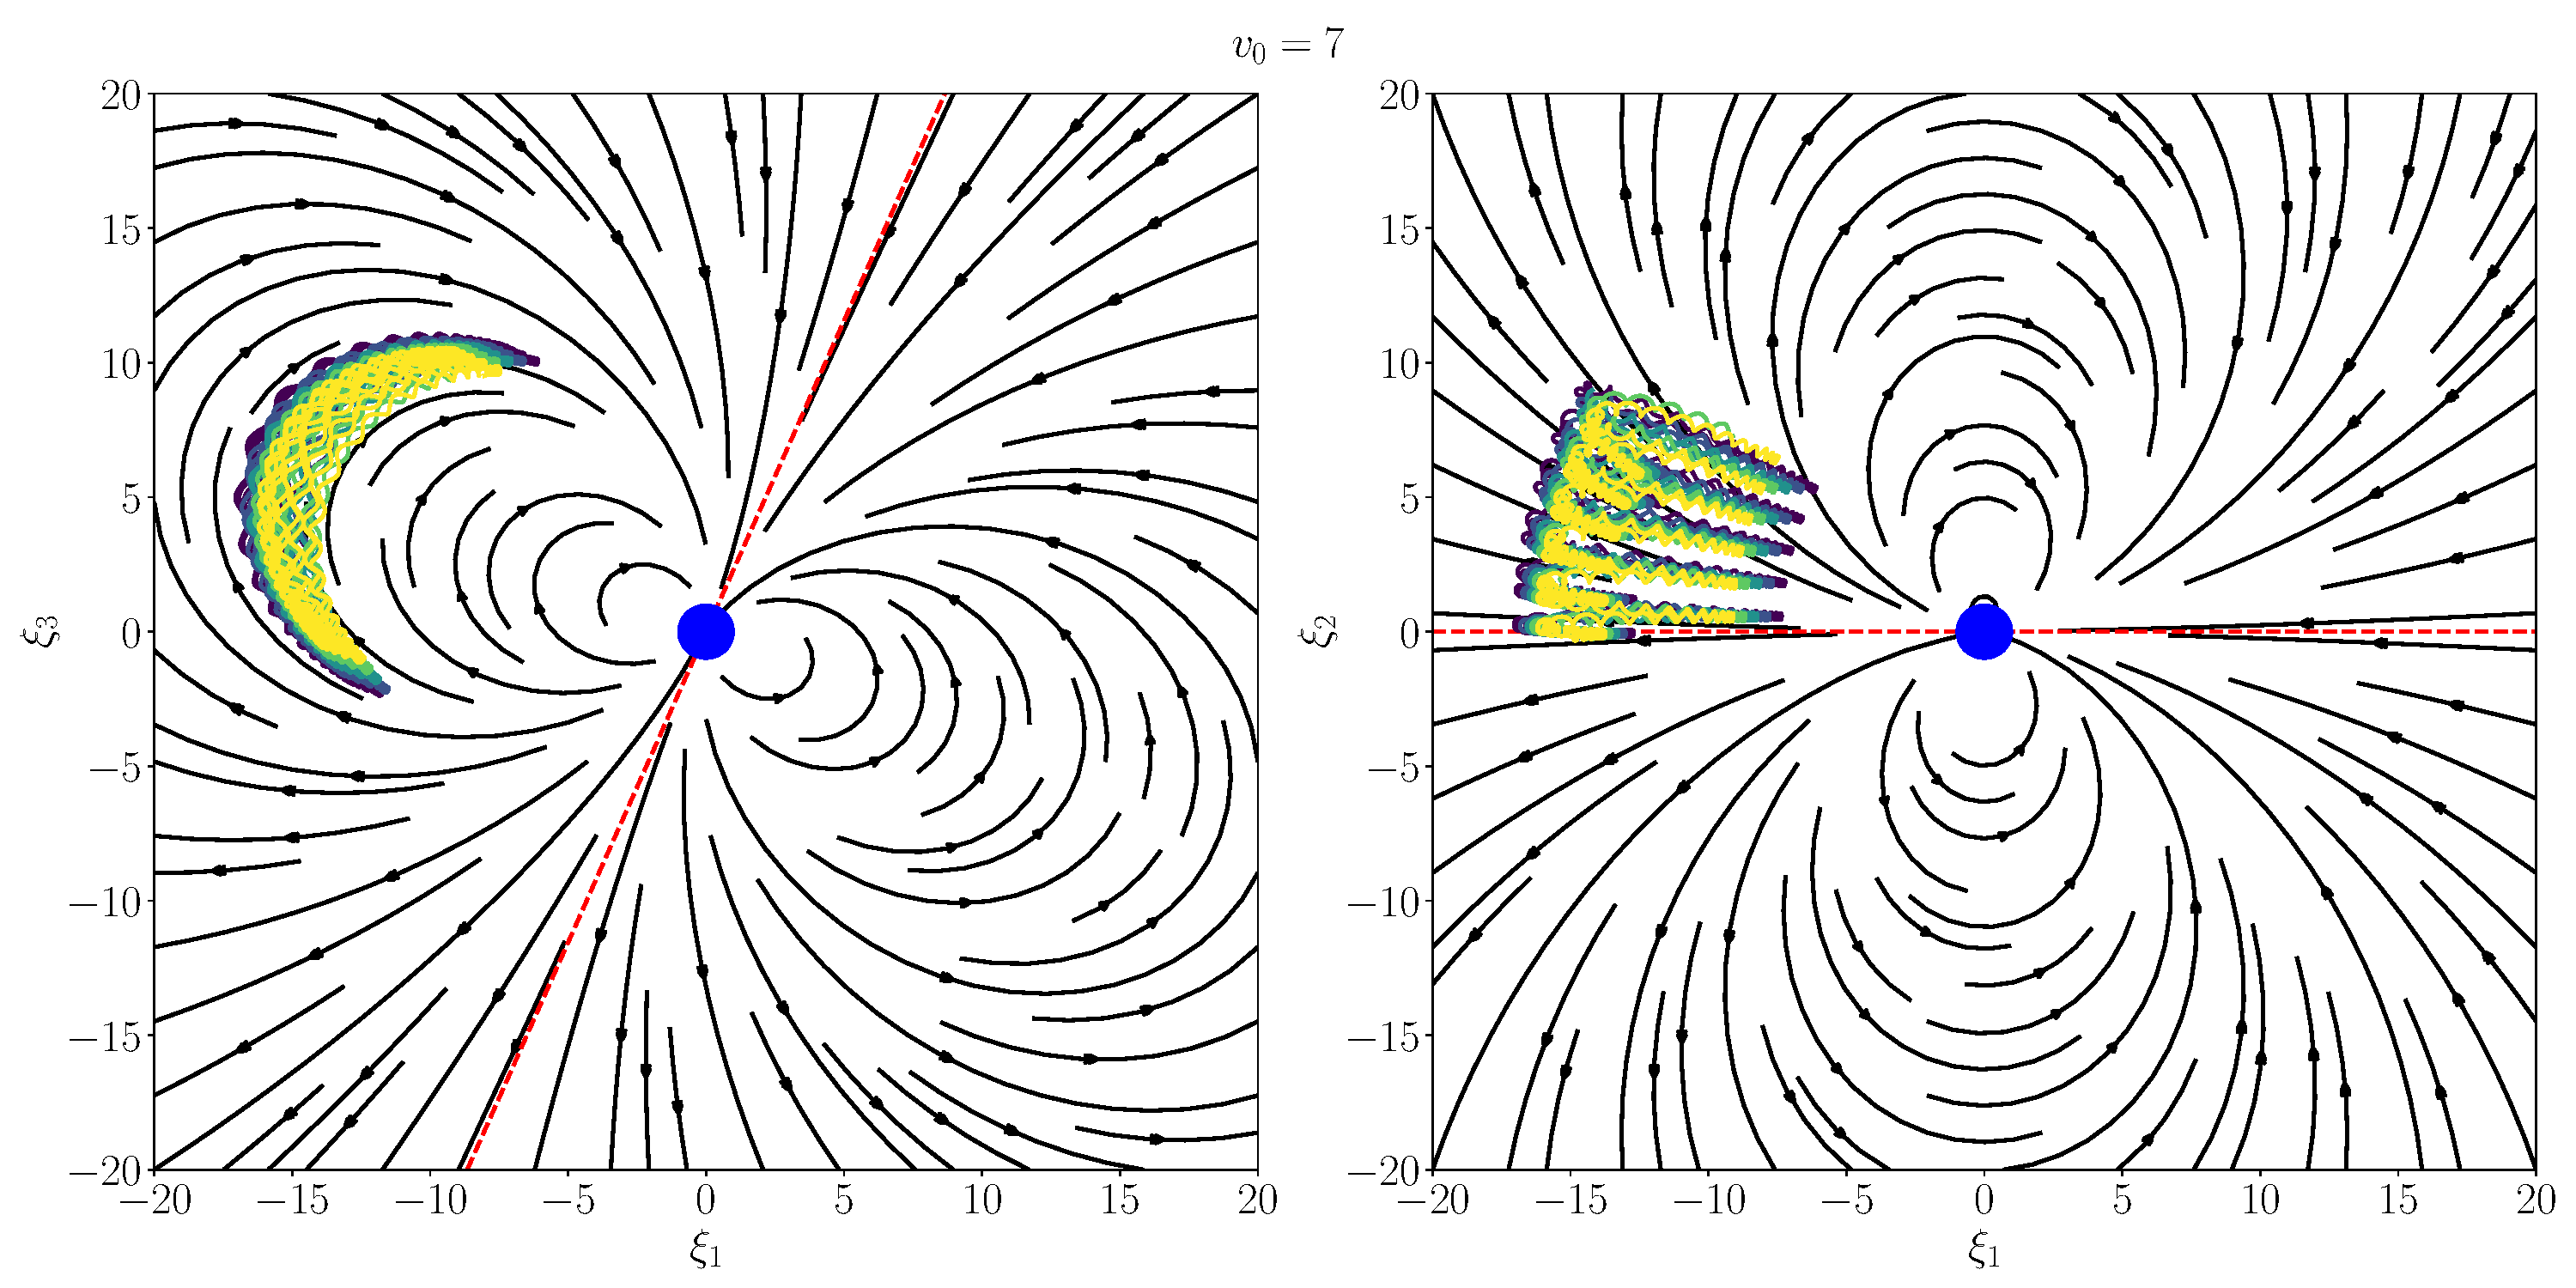
\includegraphics[width=\columnwidth]{../fig/traj_diffz.pdf}
	\caption{Particle sent towards the earth with typical solar wind velocity, for different heights $z_0$.}
	\label{fig:different_z}
\end{figure}

When doing this exact same simulation but with a weaker field ($\hat{B} \to 1/100 \hat{B}$) we observe that the same qualitative behaviour is captured. Moreover, we see here more clearly that the particles tend to spiral in towards the poles. This is exactly what causes the Aurora to be visible here and not near the equator. Note however that the strength of this field has nothing to do with that of earth's, so this demonstration is therefore not to be taken too seriously.

\begin{figure}[htb]
	\centering
	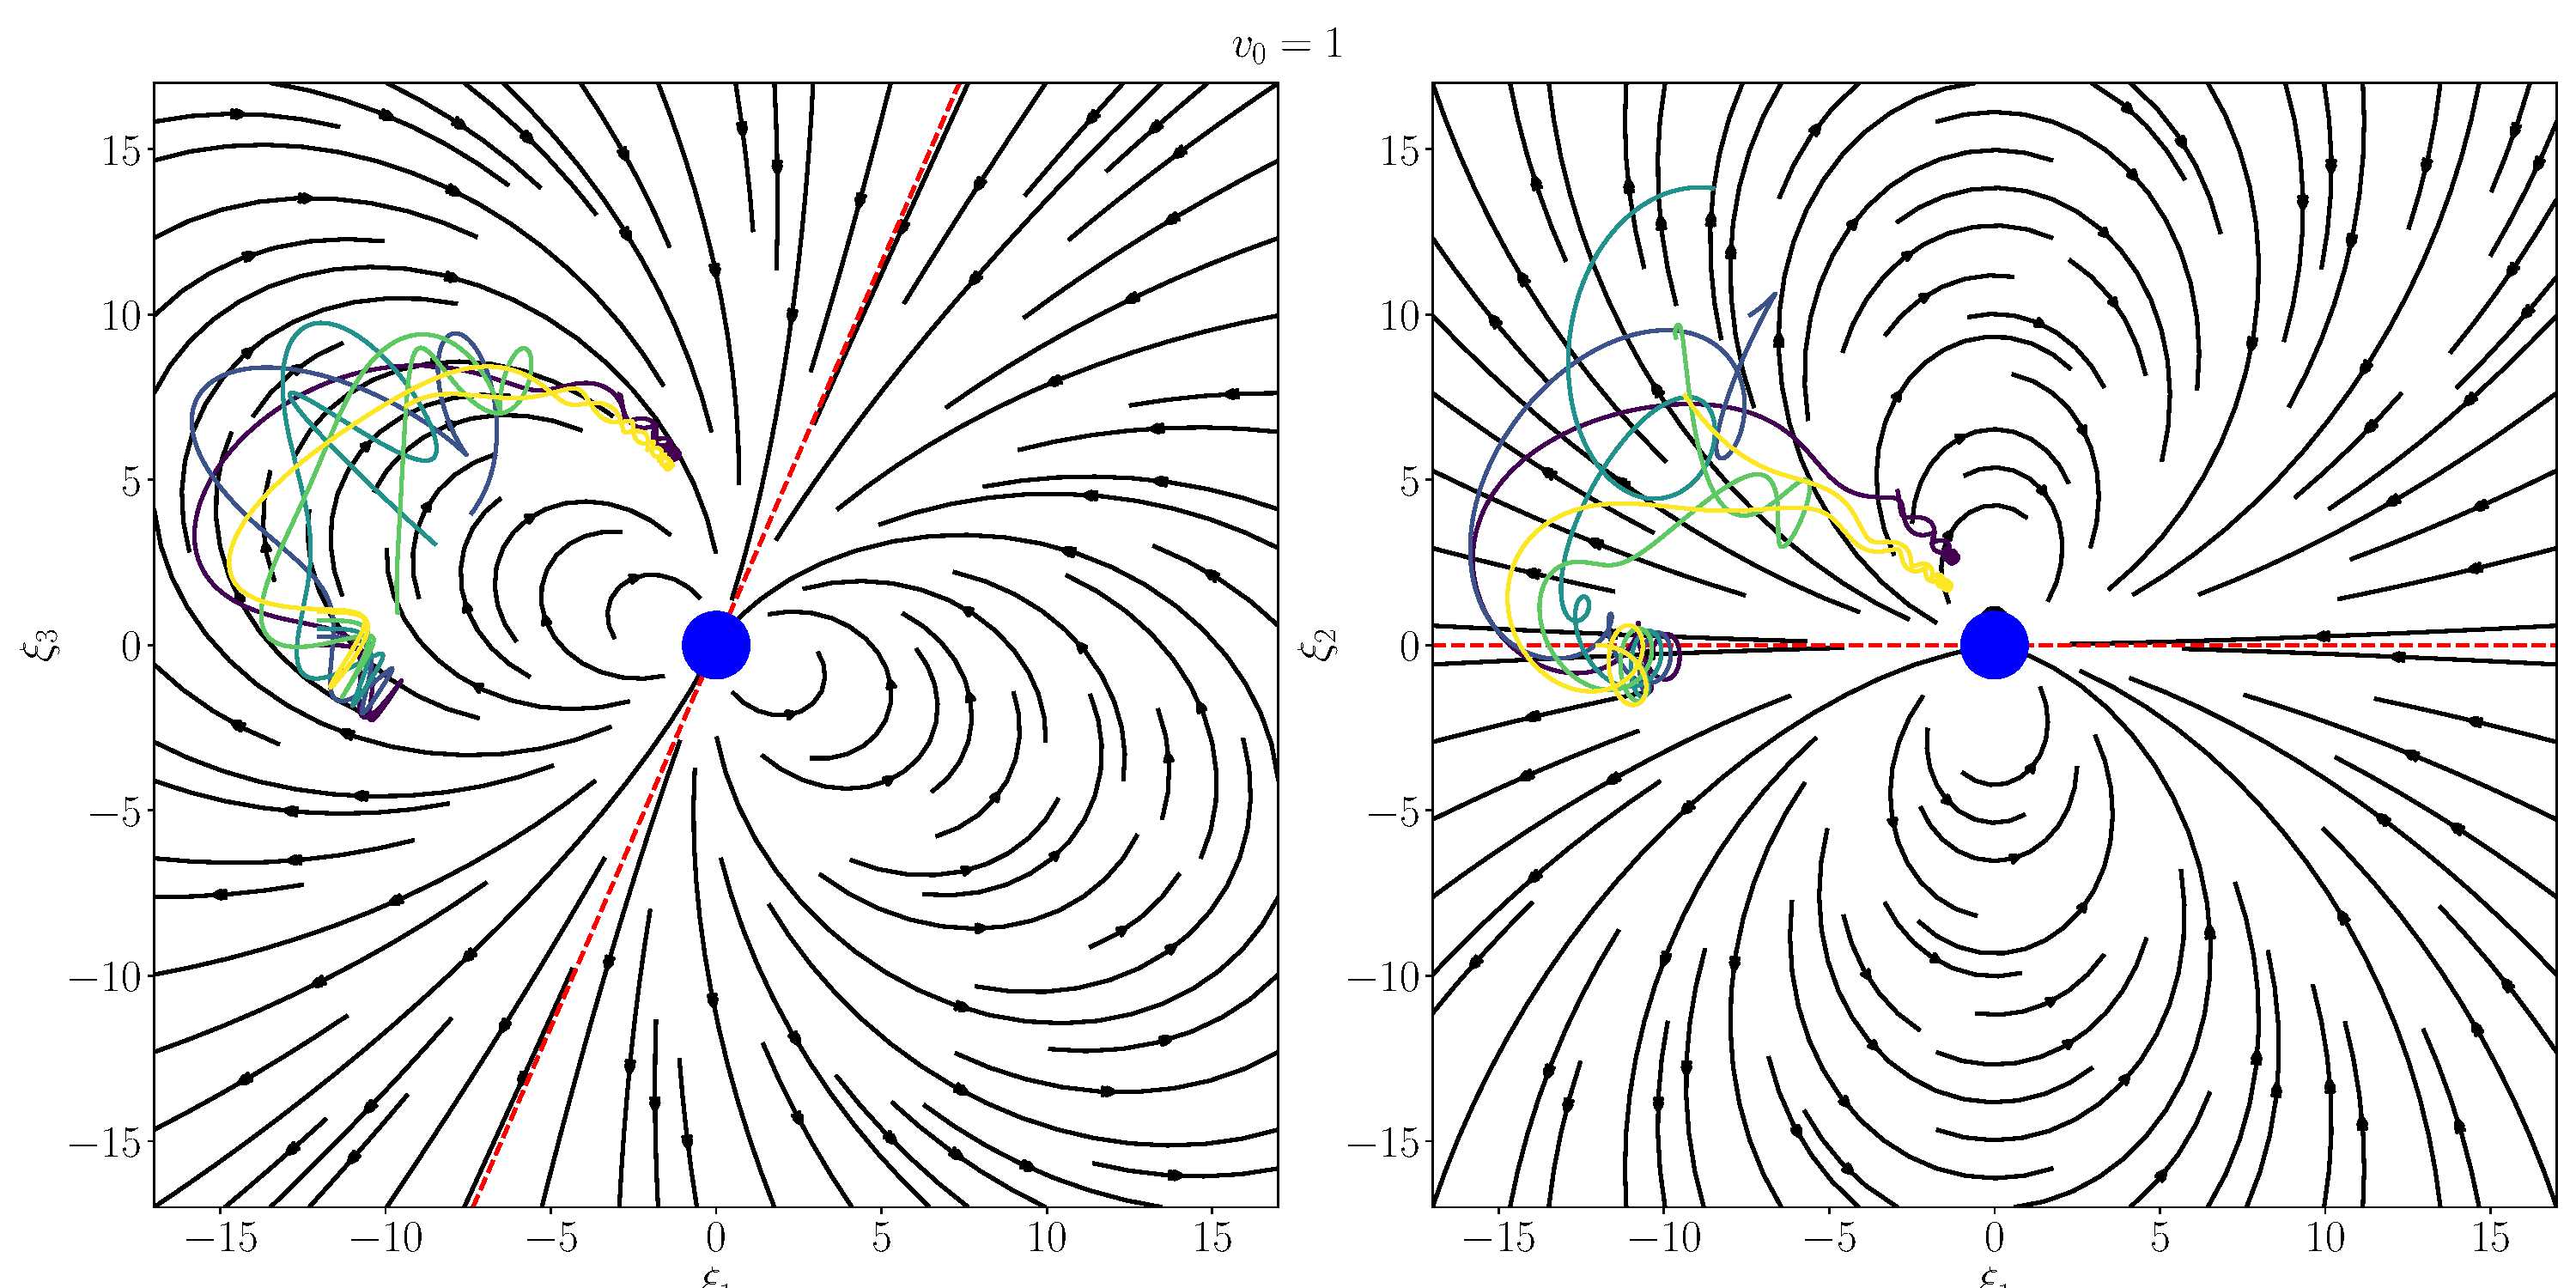
\includegraphics[width=\columnwidth]{../fig/weak_traj_diffz.pdf}
	\caption{Particle sent towards the earth with lower typical solar wind velocity, for different heights $z_0$, with a weaker field.}
	\label{fig:weak_different_z}
\end{figure}

\subsection{Validity of solution}

To have an idea of how good the numerical solution is we investigate how well energy is conserved for the particles. Since magnetic forces do no work, the energy should be invariant. The (normalised) energy difference as a function of time is shown in figure \ref{fig:energy} for some of the paths plotted above.

\begin{figure}[htb]
	\centering
	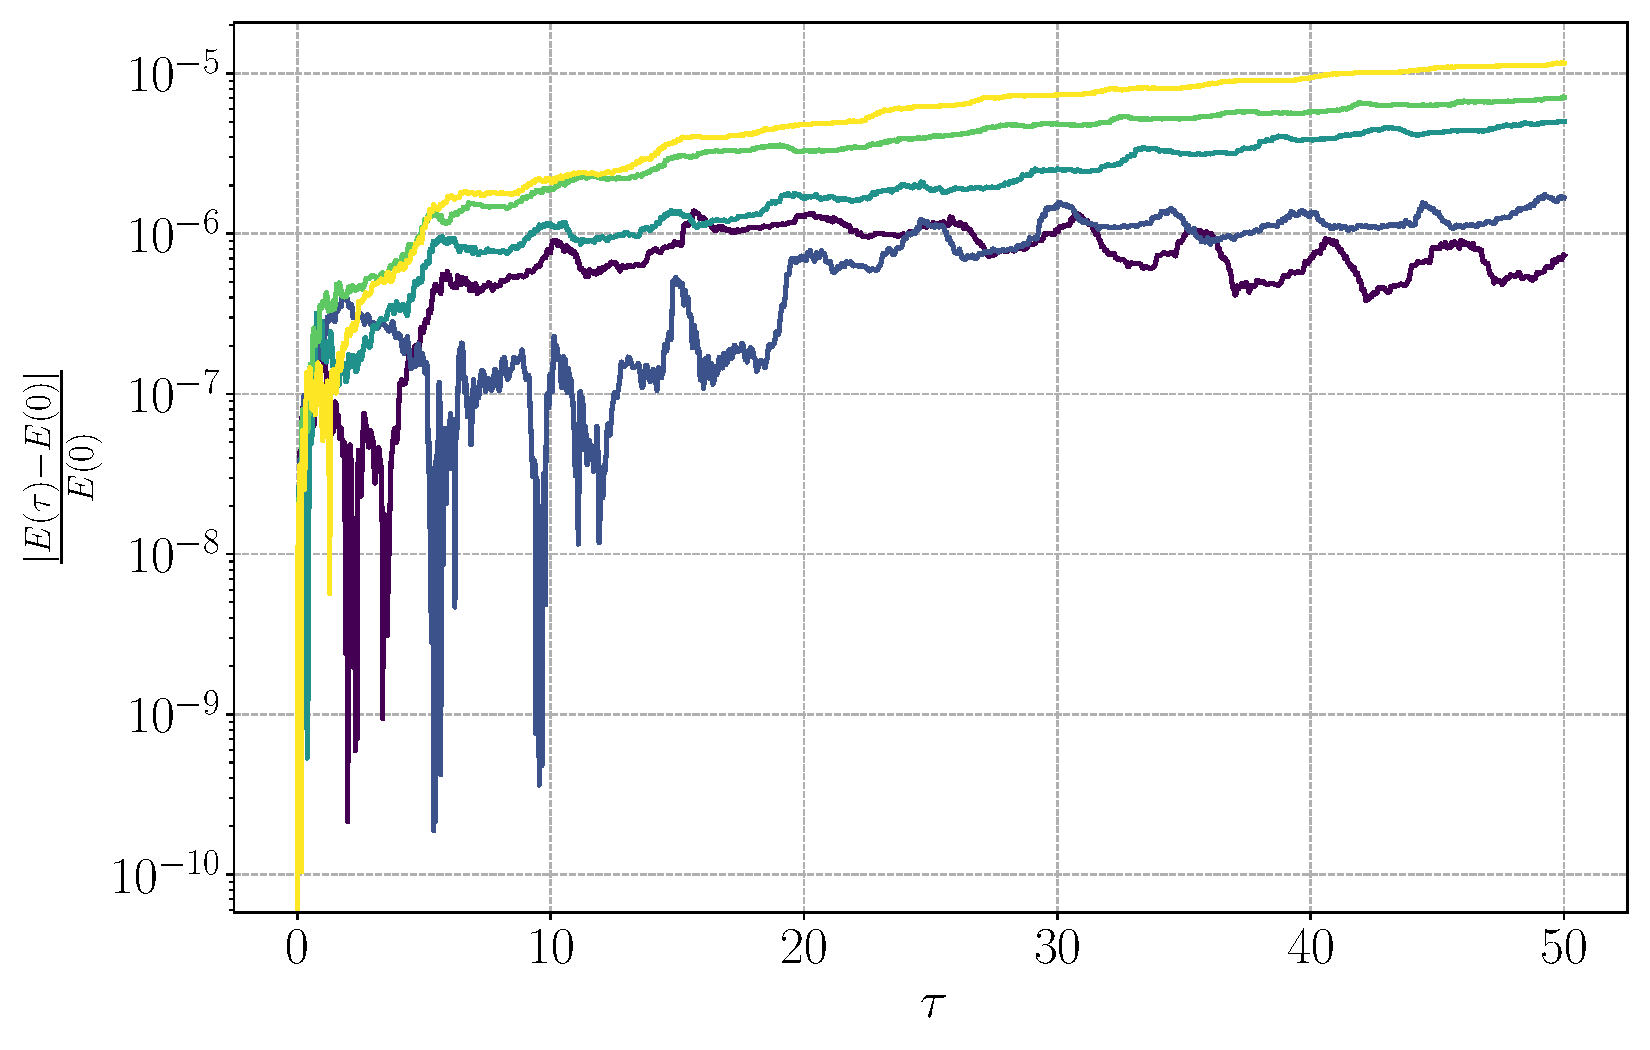
\includegraphics[width=0.8\columnwidth]{../fig/energy.pdf}
	\caption{Energy difference as a function of time for the $5$ trajectories shown in figure \ref{fig:different_z}.}
	\label{fig:energy}
\end{figure}

As the variations in the energy shown in figure \ref{fig:energy} are $\ll 1$ we conclude that the numerical validity of the solutions are good. There is however a slight drift in the energy, but that is inevitable when we take into consideration numerical round-off errors. 
 